\appendix
\chapter{Documentos}
\section{Ejemplo formato EML}
\begin{lstlisting}[
    breaklines, 
    caption={Ejemplo archivo EML}, 
    label={Documento:eml_example}, 
    captionpos=b, 
    basicstyle=\scriptsize
    ]
Return-Path: <SRS0=v5D8h6=TB=rankgator.live=kelly@untroubled.org>
Delivered-To: bruce@home.untroubled.org
Received: from rankgator.live (rdns.bitacel.com [194.34.104.232])
  by pt02.futurequest.net ([69.5.6.173])
  with ESMTP via TCP; 01 May 2019 14:41:04 -0000
Message-ID: <xat683W4TM32ruh.ilcIL221JGS1tho@rankgator.live> 
From: "Arctic Pain Relief" <kelly@rankgator.live> 
Date: Wed, 01 May 2019 10:09:17 -0400 
MIME-Version: 1.0 
Subject: Are  you -part -of-- the-- world’s- biggest arthritis cover-up? 
To: "bruce@untroubled.org" <bruce@untroubled.org> 
Content-type: multipart/alternative; boundary="---=_Part_1426_87C624P49.F740FP9";
Content-Length: 1606

-----=_Part_1426_87C624P49.F740FP9
Content-Type: text/plain; format=flowed; charset="UTF-8"
Content-Transfer-Encoding: 7bit

Are you part of the world’s biggest arthritis cover-up?

http://efs5I69IX4S3elw.rankgator.live/208fdcae990695eb0665b0903677f315_8da8c95c-0101030c0001/1/

Are you part of the world’s biggest arthritis cover-up?

-----=_Part_1426_87C624P49.F740FP9
Content-Type: text/html; charset=us-ascii
Content-Transfer-Encoding: 7bit

<!DOCTYPE html PUBLIC "-//W3C//DTD HTML 4.01 Transitional//EN">
<html>
  <head>
    <title></title>
  </head>
  <body>
    <table>
      <tr>
        <td colspan='2' align='center' valign='middle' class='preview-mid'>
          <br>
          <center>
            <a href="http://sdvPL9B7FL5Hwfm.rankgator.live/208fdcae990695eb0665b0903677f315_8da8c95c-0101030c0001/1/"><img src="http://ifq7BTAN28Q1vfo.rankgator.live/images//4b128133049378e37097925975e252e1" border="0" alt=""></a>
          </center>
          <div align="center">
###STUFF##
            <font face="Verdana, Arial, Helvetica, sans-serif" size="1"><br>
            If you'd prefer not to receive future emails, <a href="http://pkvG0P5I93MHwgd.rankgator.live/208abda8ac8695eb0665b0903678f315_8da8c95c-0101030c0001/1/"><font color="#666666">Unsubscribe Here</font></a>.<br>
            616 Corporate Way, | Suite 2-5335 Valley Cottage | NY NY 10989</font>
          </div>
        </td>
      </tr>
    </table>
  </body>
</html>

<center>



<img src="http://pmsG8XP16WP5bqb.rankgator.live/2082301ea94695eb0665b090365f030b_8da8c95c-0101030c0001/2/">

-----=_Part_1426_87C624P49.F740FP9--
\end{lstlisting}
\chapter{Base de datos}
\section{Diagrama entidad relación}


\begin{figure}[H]
    \centering
    %\includegraphics[width=0.5\textwidth]{spiral}
    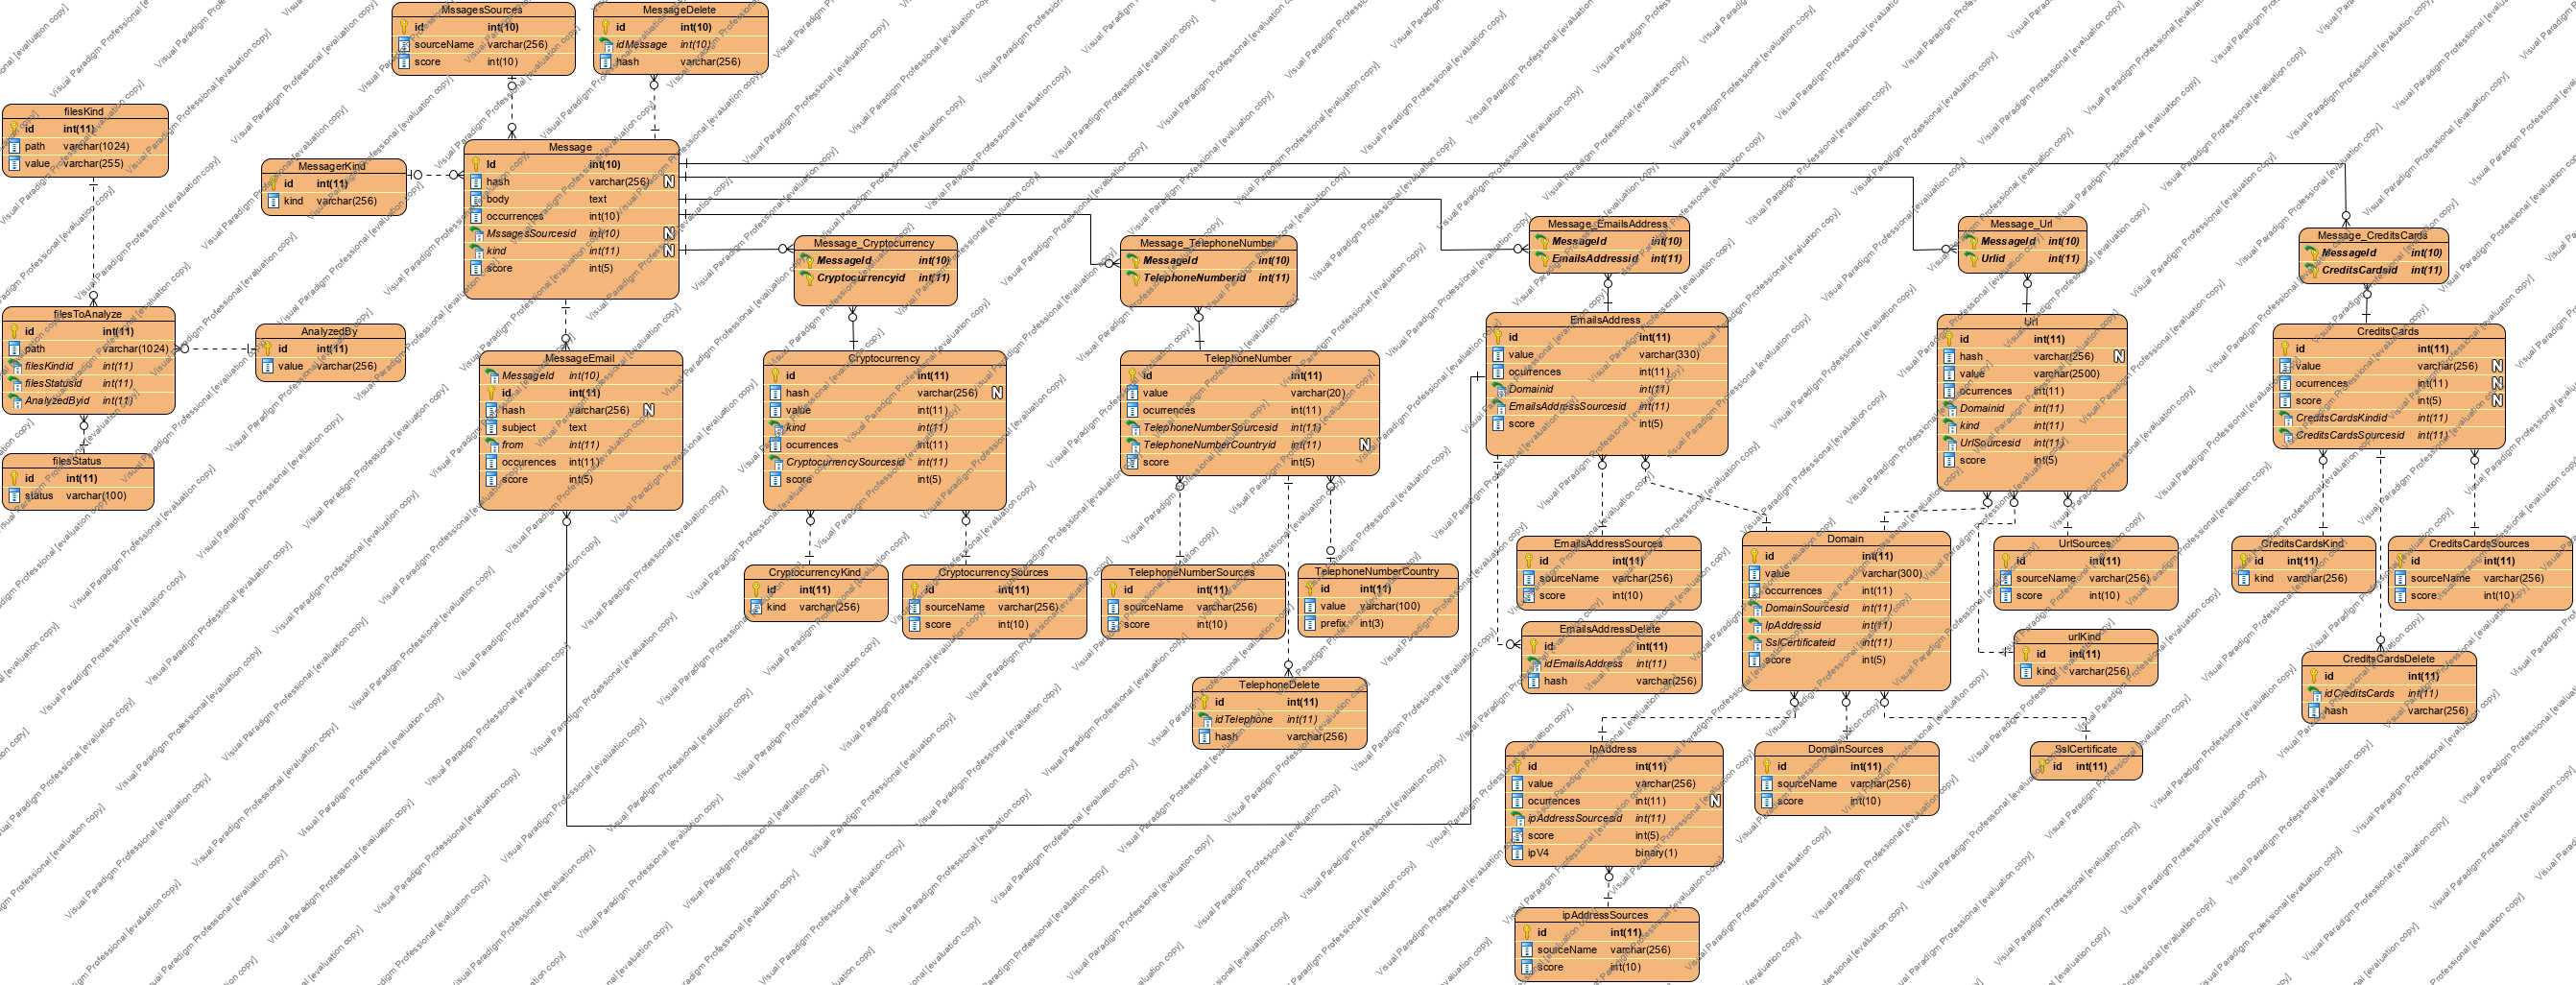
\includegraphics[scale=0.2, angle=90]{imagenes/Diagrama_entidad_relacion.png}
\caption{Diagrama entidad entidad relación de la Base de datos}
\end{figure}



\section{Tablas e índices}
\renewcommand{\lstlistingname}{Tabla}% Listing -> Algorithm

\subsection{Mensajes}
\subsubsection{Formato de los mensajes}
\begin{lstlisting}[
    language=SQL,
    breaklines, 
    caption={Tabla MessageFormat}, 
    label={Tabla:MessageFormat}, 
    basicstyle=\scriptsize,
    captionpos=b
    ]
    create  table MessageFormat (
    id   tinyint UNSIGNED  not null auto_increment, 
    value varchar(256) not null, 
    primary key (id));
    INSERT INTO MessageFormat(value) VALUES ("eml");
    INSERT INTO MessageFormat(value) VALUES ("html");
    INSERT INTO MessageFormat(value) VALUES ("text");
    INSERT INTO MessageFormat(value) VALUES ("csv");
\end{lstlisting}

\subsubsection{Analizado por}
\begin{lstlisting}[
    language=SQL,
    breaklines, 
    caption={Tabla AnalyzedBy}, 
    label={Tabla:AnalyzedBy}, 
    basicstyle=\scriptsize,
    captionpos=b
    ]
    create  table AnalyzedBy (
    id    tinyint UNSIGNED  not null auto_increment, 
    value varchar(256) not null, 
    primary key (id));
    INSERT INTO AnalyzedBy(value) VALUES ("php");
    INSERT INTO AnalyzedBy(value) VALUES ("node");
\end{lstlisting}

\subsubsection{Estado del mensaje}
\begin{lstlisting}[
    language=SQL,
    breaklines, 
    caption={Tabla MessageStatus}, 
    label={Tabla:MessageStatus}, 
    basicstyle=\scriptsize,
    captionpos=b
    ]
    create  table MessageStatus (
    id     tinyint UNSIGNED  not null auto_increment, 
    value varchar(100) not null, 
    primary key (id));
    INSERT INTO MessageStatus(value) VALUES ("pending");
    INSERT INTO MessageStatus(value) VALUES ("analyzing");
    INSERT INTO MessageStatus(value) VALUES ("analyzed");
    INSERT INTO MessageStatus(value) VALUES ("error");
\end{lstlisting}

\subsubsection{Datos del mensaje}
\begin{lstlisting}[
    language=SQL,
    breaklines, 
    caption={Tabla MessageData}, 
    label={Tabla:MessageData}, 
    basicstyle=\scriptsize,
    captionpos=b
    ]
    create  table MessageData (
    id            int UNSIGNED  not null auto_increment, 
    hash          binary(20) not null, 
    score         smallint default 0 not null, 
    format        tinyint UNSIGNED  not null, 
    analyzedBy    tinyint UNSIGNED  null DEFAULT NULL, 
    status        tinyint UNSIGNED  not null DEFAULT 1, 
    analysisTime  DECIMAL(9,6) null DEFAULT NULL,
    addeddAt      TIMESTAMP(6) NOT NULL DEFAULT CURRENT_TIMESTAMP(6),
    analyzedAt    TIMESTAMP(6) NULL DEFAULT NULL,
    updatedAt     TIMESTAMP(6) NULL DEFAULT NULL ON UPDATE CURRENT_TIMESTAMP(6),
    UNIQUE INDEX iq_messageData_hash (hash ASC),
    CONSTRAINT FK_MessageFormat_Message FOREIGN KEY (format) REFERENCES MessageFormat (id) ON DELETE NO ACTION ON UPDATE NO ACTION,
    CONSTRAINT FK_AnalyzedBy_Message FOREIGN KEY (analyzedBy) REFERENCES AnalyzedBy (id) ON DELETE NO ACTION ON UPDATE NO ACTION,
    CONSTRAINT FK_MessageStatus_Message FOREIGN KEY (status) REFERENCES MessageStatus (id) ON DELETE NO ACTION ON UPDATE NO ACTION,
    primary key (Id));
\end{lstlisting}

\subsubsection{Texto del mensaje}
\begin{lstlisting}[
    language=SQL,
    breaklines, 
    caption={Tabla MessageText}, 
    label={Tabla:MessageText}, 
    basicstyle=\scriptsize,
    captionpos=b
    ]
    create  table MessageText (
    id            int UNSIGNED  not null auto_increment, 
    value         text CHARACTER SET utf8 COLLATE utf8_unicode_ci NOT null, 
    CONSTRAINT FK_MessageData_MessageText FOREIGN KEY (id) REFERENCES MessageData (id) ON DELETE CASCADE ON UPDATE NO ACTION,
    FULLTEXT ftidx_MessageText_value (value),
    primary key (id));
\end{lstlisting}

\subsubsection{Submensajes}
\begin{lstlisting}[
    language=SQL,
    breaklines, 
    caption={Tabla ChildMessages}, 
    label={Tabla:ChildMessages}, 
    basicstyle=\scriptsize,
    captionpos=b
    ]
    create  table ChildMessages (
    parentId         int UNSIGNED  not null, 
    childId          int UNSIGNED  not null, 
    CONSTRAINT FK_MessageData_Message_ChildMessages_Parent FOREIGN KEY (parentId) REFERENCES MessageData (id) ON DELETE CASCADE ON UPDATE NO ACTION,
    CONSTRAINT FK_MessageData_Message_ChildMessages_Child FOREIGN KEY (childId) REFERENCES MessageData (id) ON DELETE CASCADE ON UPDATE NO ACTION,
    primary key (parentId, childId));
\end{lstlisting}

\subsection{Patrones}

\begin{lstlisting}[
    language=SQL,
    breaklines, 
    caption={Tablas de la información extraida y auxiliares}, 
    label={Tabla:elements}, 
    basicstyle=\scriptsize,
    captionpos=b
    ]
    create  table IpAddress (
  id         int UNSIGNED  not null auto_increment, 
  hash       binary(20) not null, 
  value      varchar(50) not null, 
  score      smallint default 0 not null, 
  ipv4       tinyint(1) not null, 
  UNIQUE INDEX  iq_IpAddress_value (value ASC),
  UNIQUE INDEX  iq_IpAddress_hash (hash ASC),
  primary key (id));

create  table Domain (
  id          int UNSIGNED  not null auto_increment, 
  hash        binary(20) not null, 
  value       varchar(330) not null, 
  score       smallint default 0 not null, 
  analyzedAt  TIMESTAMP(6) NOT NULL DEFAULT CURRENT_TIMESTAMP(6),
  parentId    int UNSIGNED  null, 
  INDEX idx_domain_parentId (parentId ASC),
  UNIQUE INDEX iq_Domain_hash (hash ASC),
  primary key (id));
  ALTER TABLE Domain ADD CONSTRAINT fk_domain_parentId_id FOREIGN KEY (parentId) REFERENCES Domain (id) ON DELETE NO ACTION ON UPDATE NO ACTION;

create  table Domain_IpAddress (
  DomainId        int UNSIGNED  not null, 
  IpAddressId     int UNSIGNED  not null,
  CONSTRAINT FK_Domain__Domain_IpAddress FOREIGN KEY (DomainId) REFERENCES Domain (id) ON DELETE CASCADE ON UPDATE NO ACTION,
  CONSTRAINT FK_IpAddress__Domain_IpAddress FOREIGN KEY (IpAddressId) REFERENCES IpAddress (id) ON DELETE CASCADE ON UPDATE NO ACTION,
  primary key (DomainId, IpAddressId));


create  table EmailAddress (
  id          int UNSIGNED  not null auto_increment, 
  hash        binary(20) not null, 
  value       varchar(330) not null, 
  score       smallint default 0 not null, 
  analyzedAt  TIMESTAMP(6) NOT NULL DEFAULT CURRENT_TIMESTAMP(6),
  domain      int UNSIGNED  not null, 
  UNIQUE INDEX  iq_EmailAddress_hash (hash ASC),
  CONSTRAINT FK_Domain__EmailAddress FOREIGN KEY (domain) REFERENCES Domain (id) ON DELETE NO ACTION ON UPDATE NO ACTION,
  primary key (id));


create  table UrlType (
  id    tinyint UNSIGNED  not null auto_increment, 
  value varchar(256) not null, 
  primary key (id));

INSERT INTO UrlType(value) VALUES ("link");
INSERT INTO UrlType(value) VALUES ("img");
INSERT INTO UrlType(value) VALUES ("video");

create  table Url (
  id          int UNSIGNED  not null auto_increment, 
  hash        binary(20) not null, 
  value       varchar(2500) not null, 
  score       smallint default 0 not null, 
  analyzedAt  TIMESTAMP(6) NOT NULL DEFAULT CURRENT_TIMESTAMP(6),
  domain      int UNSIGNED  not null, 
  type        tinyint UNSIGNED  not null, 
  UNIQUE INDEX  iq_Url_hash (hash ASC),
  CONSTRAINT FK_Domain__Url FOREIGN KEY (domain) REFERENCES Domain (id) ON DELETE NO ACTION ON UPDATE NO ACTION,
  primary key (id));

create  table MessageHeaderTypes (
  id                      mediumint UNSIGNED  not null auto_increment, 
  value                   text not null, 
  primary key (id));

create  table MessageHeaderValues (
  id                      int UNSIGNED  not null auto_increment, 
  hash                    binary(20) not null, 
  value                   text not null, 
  emailHeaderTypesId      mediumint UNSIGNED  not null, 
  UNIQUE INDEX  iq_Url_hash (hash ASC),
  INDEX idx_MessageHeaderValues_emailHeaderTypesId (emailHeaderTypesId ASC),
  CONSTRAINT FK_MessageHeaderTypes__MessageHeaderValues FOREIGN KEY (emailHeaderTypesId) REFERENCES MessageHeaderTypes (id) ON DELETE NO ACTION ON UPDATE NO ACTION,
  primary key (id));




create  table MessageDelete (
  id        int UNSIGNED  not null auto_increment, 
  idMessage int UNSIGNED  not null, 
  hash      varchar(256) not null, 
  CONSTRAINT FK_MessageData_MessageDelete FOREIGN KEY (idMessage) REFERENCES MessageData (id) ON DELETE CASCADE ON UPDATE NO ACTION,
  primary key (id));

create  table MessageDataSources (
  id         SMALLINT UNSIGNED  not null auto_increment, 
  value varchar(100) not null, 
  score      smallint default 0 not null, 
  UNIQUE INDEX uq_MessageDataSources_value (value DESC),
  primary key (id));
INSERT INTO MessageDataSources(value) VALUES ("fromWeb");
INSERT INTO MessageDataSources(value) VALUES ("onEml");


create  table MessageData_MessageDataSources (
  MessageDataId         int UNSIGNED  not null, 
  MessageDataSourcesId  SMALLINT UNSIGNED  not null,
  date              TIMESTAMP(6) NOT NULL DEFAULT CURRENT_TIMESTAMP(6),
  CONSTRAINT FK_MessageData__Message_MessageDataSources FOREIGN KEY (MessageDataId) REFERENCES MessageData (id) ON DELETE CASCADE ON UPDATE NO ACTION,
  CONSTRAINT FK_MessageDataSources__Message_MessageDataSources FOREIGN KEY (MessageDataSourcesId) REFERENCES MessageDataSources (id) ON DELETE NO ACTION ON UPDATE NO ACTION,
  primary key (MessageDataId, MessageDataSourcesId, date));






create  table IpAddressSources (
  id         smallint UNSIGNED  not null auto_increment, 
  value varchar(100) not null, 
  score      smallint  default 0 not null, 
  UNIQUE INDEX uq_IpAddressSources_value (value DESC),
  primary key (id));
INSERT INTO IpAddressSources(value) VALUES ("textAnalysis");
INSERT INTO IpAddressSources(value) VALUES ("emlHeaders");
INSERT INTO IpAddressSources(value) VALUES ("onDomain");
INSERT INTO IpAddressSources(value) VALUES ("aHref");
INSERT INTO IpAddressSources(value) VALUES ("aText");


create  table IpAddress_IpAddressSources (
  IpAddressId         int UNSIGNED  not null, 
  IpAddressSourcesId smallint UNSIGNED  not null,
  date              TIMESTAMP(6) NOT NULL DEFAULT CURRENT_TIMESTAMP(6),
  CONSTRAINT FK_IpAddress__IpAddress_IpAddressSources FOREIGN KEY (IpAddressId) REFERENCES IpAddress (id) ON DELETE CASCADE ON UPDATE NO ACTION,
  CONSTRAINT FK_IpAddressSources__IpAddress_IpAddressSources FOREIGN KEY (IpAddressSourcesId) REFERENCES IpAddressSources (id) ON DELETE NO ACTION ON UPDATE NO ACTION,
  primary key (IpAddressId, IpAddressSourcesId, date));



create  table DomainSources (
  id         smallint UNSIGNED  not null auto_increment, 
  value varchar(100) not null, 
  score      smallint  default 0 not null, 
  UNIQUE INDEX uq_DomainSources_value (value DESC),
  primary key (id));
INSERT INTO DomainSources(value) VALUES ("textAnalysis");
INSERT INTO DomainSources(value) VALUES ("emlHeaders");
INSERT INTO DomainSources(value) VALUES ("onUrl");
INSERT INTO DomainSources(value) VALUES ("onSubdomain");
INSERT INTO DomainSources(value) VALUES ("onEmailAddress");
INSERT INTO DomainSources(value) VALUES ("aHref");
INSERT INTO DomainSources(value) VALUES ("aText");

create  table Domain_DomainSources (
  DomainId          int UNSIGNED  not null, 
  DomainSourcesId   smallint UNSIGNED  not null,
  date              TIMESTAMP(6) NOT NULL DEFAULT CURRENT_TIMESTAMP(6),
  CONSTRAINT FK_Domain__Domain_DomainSources FOREIGN KEY (DomainId) REFERENCES Domain (id) ON DELETE CASCADE ON UPDATE NO ACTION,
  CONSTRAINT FK_DomainSources__Domain_DomainSources FOREIGN KEY (DomainSourcesId) REFERENCES DomainSources (id) ON DELETE NO ACTION ON UPDATE NO ACTION,
  primary key (DomainId, DomainSourcesId, date));

create  table DomainMaliciousChecks (
  id         smallint UNSIGNED  not null auto_increment, 
  value      varchar(250) not null, 
  score      smallint default 0 not null, 
  primary key (id));

create  table Domain_DomainMaliciousChecks (
  DomainId                int UNSIGNED  not null, 
  DomainMaliciousChecksId smallint UNSIGNED  not null,
  CONSTRAINT FK_Domain__Domain_DomainMaliciousChecks FOREIGN KEY (DomainId) REFERENCES Domain (id) ON DELETE CASCADE ON UPDATE NO ACTION,
  CONSTRAINT FK_DomainMaliciousChecks__Domain_DomainMaliciousChecks FOREIGN KEY (DomainMaliciousChecksId) REFERENCES DomainMaliciousChecks (id) ON DELETE NO ACTION ON UPDATE NO ACTION,
  primary key (DomainId, DomainMaliciousChecksId));




create  table EmailAddressDelete (
  id        int UNSIGNED  not null auto_increment, 
  idEmailAddress int UNSIGNED  not null, 
  hash      varchar(256) not null, 
  CONSTRAINT FK_EmailAddress_EmailAddressDelete FOREIGN KEY (idEmailAddress) REFERENCES EmailAddress (id) ON DELETE CASCADE ON UPDATE NO ACTION,
  primary key (id));

create  table EmailAddressSources (
  id         smallint UNSIGNED  not null auto_increment, 
  value varchar(100) not null, 
  score      smallint default 0 not null, 
  UNIQUE INDEX uq_EmailAddressSources_value (value DESC),
  primary key (id));
INSERT INTO EmailAddressSources(value) VALUES ("textAnalysis");
INSERT INTO EmailAddressSources(value) VALUES ("emlHeaders");
INSERT INTO EmailAddressSources(value) VALUES ("aHref");
INSERT INTO EmailAddressSources(value) VALUES ("aText");

create  table EmailAddress_EmailAddressSources (
  EmailAddressId          int UNSIGNED  not null, 
  EmailAddressSourcesId   smallint UNSIGNED  not null,
  date                    TIMESTAMP(6) NOT NULL DEFAULT CURRENT_TIMESTAMP(6),
  CONSTRAINT FK_EmailAddress__EmailAddress_EmailAddressSources FOREIGN KEY (EmailAddressId) REFERENCES EmailAddress (id) ON DELETE CASCADE ON UPDATE NO ACTION,
  CONSTRAINT FK_EmailAddressSources__EmailAddress_EmailAddressSources FOREIGN KEY (EmailAddressSourcesId) REFERENCES EmailAddressSources (id) ON DELETE NO ACTION ON UPDATE NO ACTION,
  primary key (EmailAddressId, EmailAddressSourcesId, date));

create  table EmailAddressMaliciousChecks (
  id         smallint UNSIGNED  not null auto_increment, 
  value      varchar(250) not null, 
  score      smallint default 0 not null, 
  primary key (id));

create  table EmailAddress_EmailAddressMaliciousChecks (
  EmailAddressId                int UNSIGNED  not null, 
  EmailAddressMaliciousChecksId smallint UNSIGNED  not null,
  CONSTRAINT FK_EmailAddress__EmailAddress_EmailAddressMaliciousChecks FOREIGN KEY (EmailAddressId) REFERENCES EmailAddress (id) ON DELETE CASCADE ON UPDATE NO ACTION,
  CONSTRAINT FK_EmailAddressMC__EmailAddress_EmailAddressMC FOREIGN KEY (EmailAddressMaliciousChecksId) REFERENCES EmailAddressMaliciousChecks (id) ON DELETE NO ACTION ON UPDATE NO ACTION,
  primary key (EmailAddressId, EmailAddressMaliciousChecksId));
  
create  table EmailAddress_href_value (
  href         int UNSIGNED  not null, 
  text          int UNSIGNED  not null, 
  CONSTRAINT FK_EmailAddress__EmailAddress_href_value_href FOREIGN KEY (href) REFERENCES EmailAddress (id) ON DELETE CASCADE ON UPDATE NO ACTION,
  CONSTRAINT FK_EmailAddress__EmailAddress_href_value_text FOREIGN KEY (text) REFERENCES EmailAddress (id) ON DELETE CASCADE ON UPDATE NO ACTION,
  primary key (href, text));




create  table MessageData_IpAddress (
  MessageDataId   int UNSIGNED  not null, 
  IpAddressId     int UNSIGNED  not null,
  CONSTRAINT FK_MessageData__MessageData_IpAddress FOREIGN KEY (MessageDataId) REFERENCES MessageData (id) ON DELETE CASCADE ON UPDATE NO ACTION,
  CONSTRAINT FK_IpAddress__MessageData_IpAddress FOREIGN KEY (IpAddressId) REFERENCES IpAddress (id) ON DELETE NO ACTION ON UPDATE NO ACTION,
  primary key (MessageDataId, IpAddressId));

create  table MessageData_Domain (
  MessageDataId      int UNSIGNED  not null, 
  DomainId           int UNSIGNED  not null,
  CONSTRAINT FK_MessageData__MessageData_Domain FOREIGN KEY (MessageDataId) REFERENCES MessageData (id) ON DELETE CASCADE ON UPDATE NO ACTION,
  CONSTRAINT FK_Domain__MessageData_Domain FOREIGN KEY (DomainId) REFERENCES Domain (id) ON DELETE NO ACTION ON UPDATE NO ACTION,
  primary key (MessageDataId, DomainId));

create  table MessageData_EmailAddress (
  MessageDataId      int UNSIGNED  not null, 
  EmailAddressId     int UNSIGNED  not null,
  CONSTRAINT FK_MessageData__MessageData_EmailAddress FOREIGN KEY (MessageDataId) REFERENCES MessageData (id) ON DELETE CASCADE ON UPDATE NO ACTION,
  CONSTRAINT FK_EmailAddress__MessageData_EmailAddress FOREIGN KEY (EmailAddressId) REFERENCES EmailAddress (id) ON DELETE NO ACTION ON UPDATE NO ACTION,
  primary key (MessageDataId, EmailAddressId));

create  table MessageData_Url (
  MessageDataId     int UNSIGNED  not null, 
  UrlId             int UNSIGNED  not null,
  CONSTRAINT FK_MessageData__MessageData_Url FOREIGN KEY (MessageDataId) REFERENCES MessageData (id) ON DELETE CASCADE ON UPDATE NO ACTION,
  CONSTRAINT FK_Url__MessageData_Url FOREIGN KEY (UrlId) REFERENCES Url (id) ON DELETE NO ACTION ON UPDATE NO ACTION,
  primary key (MessageDataId, UrlId));

create  table MessageData_MessageHeaderValues (
  MessageDataId         int UNSIGNED  not null, 
  MessageHeaderValuesId int UNSIGNED  not null,
  CONSTRAINT FK_MessageData__MessageData_MessageHeaderValues FOREIGN KEY (MessageDataId) REFERENCES MessageData (id) ON DELETE CASCADE ON UPDATE NO ACTION,
  CONSTRAINT FK_MessageHeaderValues__MessageData_MessageHeaderValues FOREIGN KEY (MessageHeaderValuesId) REFERENCES MessageHeaderValues (id) ON DELETE NO ACTION ON UPDATE NO ACTION,
  primary key (MessageDataId, MessageHeaderValuesId));




create  table UrlSources (
  id         smallint UNSIGNED  not null auto_increment, 
  value      varchar(100) not null, 
  score      smallint  default 0 not null, 
  UNIQUE INDEX uq_UrlSources_value (value DESC),
  primary key (id));
INSERT INTO UrlSources(value) VALUES ("textAnalysis");
INSERT INTO UrlSources(value) VALUES ("emlHeaders");
INSERT INTO UrlSources(value) VALUES ("aHref");
INSERT INTO UrlSources(value) VALUES ("aText");

create  table Url_UrlSources (
  UrlId         int UNSIGNED  not null, 
  UrlSourcesId  smallint UNSIGNED  not null,
  date          TIMESTAMP(6) NOT NULL DEFAULT CURRENT_TIMESTAMP(6),
  CONSTRAINT FK_Url__Url_UrlSources FOREIGN KEY (UrlId) REFERENCES Url (id) ON DELETE CASCADE ON UPDATE NO ACTION,
  CONSTRAINT FK_UrlSources__Url_UrlSources FOREIGN KEY (UrlSourcesId) REFERENCES UrlSources (id) ON DELETE NO ACTION ON UPDATE NO ACTION,
  primary key (UrlId, UrlSourcesId, date));

create  table UrlMaliciousChecks (
  id         smallint UNSIGNED  not null auto_increment, 
  value      varchar(250) not null, 
  score      smallint default 0 not null, 
  primary key (id));

create  table Url_UrlMaliciousChecks (
  UrlId                 int UNSIGNED  not null, 
  UrlMaliciousChecksId  smallint UNSIGNED  not null,
  CONSTRAINT FK_Url__Url_UrlMaliciousChecks FOREIGN KEY (UrlId) REFERENCES Url (id) ON DELETE CASCADE ON UPDATE NO ACTION,
  CONSTRAINT FK_UrlMaliciousChecks__Url_UrlMaliciousChecks FOREIGN KEY (UrlMaliciousChecksId) REFERENCES UrlMaliciousChecks (id) ON DELETE NO ACTION ON UPDATE NO ACTION,
  primary key (UrlId, UrlMaliciousChecksId));
  
create  table Url_href_value (
  href          int UNSIGNED  not null, 
  text          int UNSIGNED  not null, 
  CONSTRAINT FK_Url__Url_href_value_href FOREIGN KEY (href) REFERENCES Url (id) ON DELETE CASCADE ON UPDATE NO ACTION,
  CONSTRAINT FK_Url__Url_href_value_text FOREIGN KEY (text) REFERENCES Url (id) ON DELETE CASCADE ON UPDATE NO ACTION,
  primary key (href, text));



create  table MessageHeaderValues_IpAddress (
  MessageHeaderValuesId     int UNSIGNED  not null, 
  IpAddressId               int UNSIGNED  not null,
  CONSTRAINT FK_MessageHeaderValues__MessageHeaderValues_IpAddress FOREIGN KEY (MessageHeaderValuesId) REFERENCES MessageHeaderValues (id) ON DELETE CASCADE ON UPDATE NO ACTION,
  CONSTRAINT FK_IpAddress__MessageHeaderValues_IpAddress FOREIGN KEY (IpAddressId) REFERENCES IpAddress (id) ON DELETE NO ACTION ON UPDATE NO ACTION,
  primary key (MessageHeaderValuesId, IpAddressId));

create  table MessageHeaderValues_Domain (
  MessageHeaderValuesId     int UNSIGNED  not null, 
  DomainId                  int UNSIGNED  not null,
  CONSTRAINT FK_MessageHeaderValues__MessageHeaderValues_Domain FOREIGN KEY (MessageHeaderValuesId) REFERENCES MessageHeaderValues (id) ON DELETE CASCADE ON UPDATE NO ACTION,
  CONSTRAINT FK_Domain__MessageHeaderValues_Domain FOREIGN KEY (DomainId) REFERENCES Domain (id) ON DELETE NO ACTION ON UPDATE NO ACTION,
  primary key (MessageHeaderValuesId, DomainId));

create  table MessageHeaderValues_Url (
  MessageHeaderValuesId     int UNSIGNED  not null, 
  UrlId                     int UNSIGNED  not null,
  CONSTRAINT FK_MessageHeaderValues__MessageHeaderValues_Url FOREIGN KEY (MessageHeaderValuesId) REFERENCES MessageHeaderValues (id) ON DELETE CASCADE ON UPDATE NO ACTION,
  CONSTRAINT FK_Url__MessageHeaderValues_Url FOREIGN KEY (UrlId) REFERENCES Url (id) ON DELETE NO ACTION ON UPDATE NO ACTION,
  primary key (MessageHeaderValuesId, UrlId));

create  table MessageHeaderValues_EmailAddress (
  MessageHeaderValuesId     int UNSIGNED  not null, 
  EmailAddressId            int UNSIGNED  not null,
  CONSTRAINT FK_MessageHeaderValues__MessageHeaderValues_EmailAddress FOREIGN KEY (MessageHeaderValuesId) REFERENCES MessageHeaderValues (id) ON DELETE CASCADE ON UPDATE NO ACTION,
  CONSTRAINT FK_EmailAddress__MessageHeaderValues_EmailAddress FOREIGN KEY (EmailAddressId) REFERENCES EmailAddress (id) ON DELETE NO ACTION ON UPDATE NO ACTION,
  primary key (MessageHeaderValuesId, EmailAddressId));
\end{lstlisting}

\section{Vistas}
\renewcommand{\lstlistingname}{Vista}% Listing -> Algorithm

\begin{lstlisting}[
  language=SQL,
  breaklines, 
  caption={Vista MessageText\_view}, 
  label={vista:MessageTextview}, 
  basicstyle=\scriptsize,
  captionpos=b
  ]
  CREATE OR REPLACE VIEW MessageText_view AS 
  SELECT	MessageData.hash as hash, 
          MessageText.value as value, 
          MessageData.score as score, 
          MessageFormat.value as format, 
          AnalyzedBy.value as analyzedBy, 
          MessageStatus.value as status, 
          MessageData.analysisTime as analysisTime, 
          MessageData.addeddAt as addeddAt, 
          MessageData.analyzedAt as analyzedAt, 
          MessageData.updatedAt as updatedAt,
          COUNT(MessageData_MessageDataSources.MessageDataId) AS ocurrences 
  FROM MessageData 
      INNER JOIN MessageFormat ON MessageData.format = MessageFormat.id
      INNER JOIN MessageStatus ON MessageData.status = MessageStatus.id
      LEFT JOIN AnalyzedBy ON MessageData.analyzedBy = AnalyzedBy.id
      INNER JOIN MessageText on MessageData.id = MessageText.id
      INNER JOIN MessageData_MessageDataSources ON MessageData.id = MessageData_MessageDataSources.MessageDataId
  GROUP BY hash;
\end{lstlisting}

\begin{lstlisting}[
  language=SQL,
  breaklines, 
  caption={Vista MessageData\_view}, 
  label={vista:MessageDataview}, 
  basicstyle=\scriptsize,
  captionpos=b
  ]
  CREATE OR REPLACE VIEW MessageData_view AS 
  SELECT	MessageData.id as id, 
          MessageData.hash as hash, 
          MessageData.score as score, 
          MessageFormat.value as format, 
          AnalyzedBy.value as analyzedBy, 
          MessageStatus.value as status, 
          MessageData.analysisTime as analysisTime, 
          MessageData.addeddAt as addeddAt, 
          MessageData.analyzedAt as analyzedAt, 
          MessageData.updatedAt as updatedAt,
          COUNT(MessageData_MessageDataSources.MessageDataId) AS ocurrences 
  FROM MessageData 
      INNER JOIN MessageFormat ON MessageData.format = MessageFormat.id
      INNER JOIN MessageStatus ON MessageData.status = MessageStatus.id
      LEFT JOIN AnalyzedBy ON MessageData.analyzedBy = AnalyzedBy.id
      INNER JOIN MessageData_MessageDataSources ON MessageData.id = MessageData_MessageDataSources.MessageDataId
  GROUP BY hash;
\end{lstlisting}

\begin{lstlisting}[
  language=SQL,
  breaklines, 
  caption={Vista IpAddress\_view}, 
  label={vista:IpAddress_view}, 
  basicstyle=\scriptsize,
  captionpos=b
  ]
  CREATE OR REPLACE VIEW IpAddress_view AS 
  SELECT  IpAddress.id as id, 
          IpAddress.value as value, 
          IpAddress.hash as hash, 
          IpAddress.score as score, 
          IpAddress.ipv4 as ipv4, 
          COUNT(IpAddress_IpAddressSources.IpAddressId) AS ocurrences  
  FROM IpAddress
      INNER JOIN IpAddress_IpAddressSources ON IpAddress_IpAddressSources.IpAddressId = IpAddress.id GROUP BY(IpAddress.value);

\end{lstlisting}

\begin{lstlisting}[
  language=SQL,
  breaklines, 
  caption={Vista Domain\_view}, 
  label={vista:Domain_view}, 
  basicstyle=\scriptsize,
  captionpos=b
  ]
  CREATE OR REPLACE VIEW Domain_view AS 
  SELECT  Domain.id as id, 
          Domain.value as value, 
          Domain.hash as hash, 
          Domain.score as score, 
          d.value as parentDomain,
          d.hash as parentDomainHash,
          COUNT(Domain_DomainSources.DomainId) AS ocurrences  
  FROM Domain
      LEFT JOIN Domain as d ON d.id = Domain.parentId
      INNER JOIN Domain_DomainSources ON Domain_DomainSources.DomainId = Domain.id GROUP BY(Domain.value);

\end{lstlisting}

\begin{lstlisting}[
  language=SQL,
  breaklines, 
  caption={Vista domain\_ip}, 
  label={vista:domain_ip}, 
  basicstyle=\scriptsize,
  captionpos=b
  ]
  CREATE OR REPLACE  VIEW domain_ip AS 
  SELECT  Domain.value as domain,
          Domain.hash as domainHash, 
          ip.value as ip,
          ip.hash as ipHash, 
          ip.score as score
  FROM Domain
      LEFT JOIN Domain_IpAddress ON Domain.id = Domain_IpAddress.DomainId
      INNER JOIN IpAddress as ip ON ip.id = Domain_IpAddress.IpAddressId;
\end{lstlisting}

\begin{lstlisting}[
  language=SQL,
  breaklines, 
  caption={Vista subdomain}, 
  label={vista:subdomain}, 
  basicstyle=\scriptsize,
  captionpos=b
  ]
  CREATE OR REPLACE  VIEW subdomain AS 
  SELECT  Domain.value as domain, 
          Domain.hash as domainHash, 
          d.value as subdomain, 
          d.hash as subdomainHash, 
          d.score as score, 
          d.analyzedAt as analyzedAt 
  FROM Domain 
      LEFT JOIN Domain as d on d.parentId = Domain.id;
\end{lstlisting}

\begin{lstlisting}[
  language=SQL,
  breaklines, 
  caption={Vista IpAddress\_MessageData}, 
  label={vista:IpAddress_MessageData}, 
  basicstyle=\scriptsize,
  captionpos=b
  ]
  CREATE OR REPLACE VIEW IpAddress_MessageData AS 
  SELECT IpAddress.value as value,
      IpAddress.hash as IpAddressHash, 
  MessageData.hash as messageHash,
    MessageData.score as score,
      MessageFormat.value as format,
    MessageStatus.value as status,
      MessageData.addeddAt as addeddAt,
    MessageData.analyzedAt as analyzedAt
FROM IpAddress 
    LEFT JOIN MessageData_IpAddress ON IpAddress.id = MessageData_IpAddress.IpAddressId
    INNER JOIN MessageData ON MessageData.id = MessageData_IpAddress.MessageDataId
      LEFT JOIN MessageStatus ON MessageData.status = MessageStatus.id
      LEFT JOIN MessageFormat ON MessageFormat.id = MessageData.format;
\end{lstlisting}

\begin{lstlisting}[
  language=SQL,
  breaklines, 
  caption={Vista ip\_domain}, 
  label={vista:ip_domain}, 
  basicstyle=\scriptsize,
  captionpos=b
  ]
  CREATE OR REPLACE  VIEW ip_domain AS 
  SELECT  ip.value as ip, 
          ip.hash as ipHash, 
          Domain.value as domain,
          Domain.hash as domainHash, 
          Domain.score as score,
          Domain.analyzedAt as analyzedAt
  FROM IpAddress as ip 
      LEFT JOIN Domain_IpAddress ON ip.id = Domain_IpAddress.IpAddressId
      INNER JOIN Domain ON Domain.id = Domain_IpAddress.DomainId;
\end{lstlisting}

\begin{lstlisting}[
  language=SQL,
  breaklines, 
  caption={Vista Domain\_MessageData}, 
  label={vista:Domain_MessageData}, 
  basicstyle=\scriptsize,
  captionpos=b
  ]
  CREATE OR REPLACE VIEW Domain_MessageData AS 
  SELECT Domain.value as value,
      Domain.hash as DomainHash, 
  MessageData.hash as messageHash,
    MessageData.score as score,
      MessageFormat.value as format,
    MessageStatus.value as status,
      MessageData.addeddAt as addeddAt,
    MessageData.analyzedAt as analyzedAt
FROM Domain 
    LEFT JOIN MessageData_Domain ON Domain.id = MessageData_Domain.DomainId
    INNER JOIN MessageData ON MessageData.id = MessageData_Domain.MessageDataId
      LEFT JOIN MessageStatus ON MessageData.status = MessageStatus.id
      LEFT JOIN MessageFormat ON MessageFormat.id = MessageData.format;
\end{lstlisting}

\begin{lstlisting}[
  language=SQL,
  breaklines, 
  caption={Vista domain\_url}, 
  label={vista:domain_url}, 
  basicstyle=\scriptsize,
  captionpos=b
  ]
  CREATE OR REPLACE VIEW domain_url AS 
  SELECT  Domain.value as domain, 
          Domain.hash as domainHash, 
          Url.value as url,
          Url.hash as urlHash, 
          Url.score as score,
          Url.analyzedAt as analyzedAt
  FROM Domain 
      INNER JOIN Url ON Domain.id = Url.domain;
\end{lstlisting}

\begin{lstlisting}[
  language=SQL,
  breaklines, 
  caption={Vista domain\_email}, 
  label={vista:domain_email}, 
  basicstyle=\scriptsize,
  captionpos=b
  ]
  CREATE OR REPLACE VIEW domain_email AS 
  SELECT  Domain.value as domain, 
          Domain.id as id,
          Domain.hash as domainHash, 
          EmailAddress.value as email,
          EmailAddress.hash as emailAddressHash, 
          EmailAddress.score as score,
          EmailAddress.analyzedAt as analyzedAt
  FROM Domain 
      INNER JOIN EmailAddress ON Domain.id = EmailAddress.domain;
\end{lstlisting}

\begin{lstlisting}[
  language=SQL,
  breaklines, 
  caption={Vista EmailAddress\_view}, 
  label={vista:EmailAddress_view}, 
  basicstyle=\scriptsize,
  captionpos=b
  ]
  CREATE OR REPLACE VIEW EmailAddress_view AS 
  SELECT  EmailAddress.value as value, 
          EmailAddress.hash as hash, 
          EmailAddress.score as score, 
          Domain.value as domain,
          Domain.hash as domainHash, 
          COUNT(EmailAddress_EmailAddressSources.EmailAddressId) AS ocurrences  
  FROM EmailAddress
      LEFT JOIN Domain ON EmailAddress.domain = Domain.id
      INNER JOIN EmailAddress_EmailAddressSources ON EmailAddress_EmailAddressSources.EmailAddressId = EmailAddress.id GROUP BY(EmailAddress.value);
\end{lstlisting}

\begin{lstlisting}[
  language=SQL,
  breaklines, 
  caption={Vista EmailAddress\_MessageData}, 
  label={vista:EmailAddress_MessageData}, 
  basicstyle=\scriptsize,
  captionpos=b
  ]
  CREATE OR REPLACE VIEW EmailAddress_MessageData AS 
  SELECT EmailAddress.value as value,
      EmailAddress.hash as emailAddressHash, 
  MessageData.hash as messageHash,
    MessageData.score as score,
      MessageFormat.value as format,
    MessageStatus.value as status,
      MessageData.addeddAt as addeddAt,
    MessageData.analyzedAt as analyzedAt
FROM EmailAddress 
    LEFT JOIN MessageData_EmailAddress ON EmailAddress.id = MessageData_EmailAddress.EmailAddressId
    INNER JOIN MessageData ON MessageData.id = MessageData_EmailAddress.MessageDataId
      LEFT JOIN MessageStatus ON MessageData.status = MessageStatus.id
      LEFT JOIN MessageFormat ON MessageFormat.id = MessageData.format;
\end{lstlisting}

\begin{lstlisting}[
  language=SQL,
  breaklines, 
  caption={Vista Url\_view}, 
  label={vista:Url_view}, 
  basicstyle=\scriptsize,
  captionpos=b
  ]
  CREATE OR REPLACE VIEW Url_view AS 
  SELECT  Url.value as value, 
          Url.id as id,
          Url.hash as hash, 
          Url.score as score, 
          Domain.value as domain,
          Domain.hash as domainHash, 
          COUNT(Url_UrlSources.UrlId) AS ocurrences  
  FROM Url
      LEFT JOIN Domain ON Url.domain = Domain.id
      INNER JOIN Url_UrlSources ON Url_UrlSources.UrlId = Url.id GROUP BY(Url.value);
\end{lstlisting}

\begin{lstlisting}[
  language=SQL,
  breaklines, 
  caption={Vista Url\_MessageData}, 
  label={vista:Url_MessageData}, 
  basicstyle=\scriptsize,
  captionpos=b
  ]
  CREATE OR REPLACE VIEW Url_MessageData AS 
  SELECT Url.value as value,
      Url.hash as UrlHash, 
  MessageData.hash as messageHash,
    MessageData.score as score,
      MessageFormat.value as format,
    MessageStatus.value as status,
      MessageData.addeddAt as addeddAt,
    MessageData.analyzedAt as analyzedAt
FROM Url 
    LEFT JOIN MessageData_Url ON Url.id = MessageData_Url.UrlId
    INNER JOIN MessageData ON MessageData.id = MessageData_Url.MessageDataId
      LEFT JOIN MessageStatus ON MessageData.status = MessageStatus.id
      LEFT JOIN MessageFormat ON MessageFormat.id = MessageData.format;
\end{lstlisting}

\begin{lstlisting}[
  language=SQL,
  breaklines, 
  caption={Vista MessageData\_IpAddress\_view}, 
  label={vista:MessageData_IpAddress_view}, 
  basicstyle=\scriptsize,
  captionpos=b
  ]
  CREATE OR REPLACE VIEW MessageData_IpAddress_view AS 
  SELECT  MessageData.hash as hash,
       IpAddress.value AS ip, 
           IpAddress.hash as ipHash, 
           IpAddress.score as score, 
           IpAddress.ipv4 as ipv4
   FROM MessageData 
     LEFT JOIN MessageData_IpAddress ON MessageData.id = MessageData_IpAddress.MessageDataId
       INNER JOIN IpAddress ON MessageData_IpAddress.IpAddressId = IpAddress.id;
\end{lstlisting}

\begin{lstlisting}[
  language=SQL,
  breaklines, 
  caption={Vista MessageData\_EmailAddress\_view}, 
  label={vista:MessageData_EmailAddress_view}, 
  basicstyle=\scriptsize,
  captionpos=b
  ]
  CREATE OR REPLACE VIEW MessageData_EmailAddress_view AS 
  SELECT  MessageData.hash as hash,
       EmailAddress.value AS email, 
           EmailAddress.hash as emailAddressHash, 
           EmailAddress.score as score,
           Domain.value AS domain,
           Domain.hash as domainHash
   FROM MessageData 
     LEFT JOIN MessageData_EmailAddress ON MessageData.id = MessageData_EmailAddress.MessageDataId
       INNER JOIN EmailAddress ON MessageData_EmailAddress.EmailAddressId = EmailAddress.id
       INNER JOIN Domain ON EmailAddress.domain = Domain.id;
\end{lstlisting}

\begin{lstlisting}[
  language=SQL,
  breaklines, 
  caption={Vista MessageData\_Domain\_view}, 
  label={vista:MessageData_Domain_view}, 
  basicstyle=\scriptsize,
  captionpos=b
  ]
  CREATE OR REPLACE VIEW MessageData_Domain_view AS 
  SELECT  MessageData.hash as hash,
       Domain.value AS domain, 
           Domain.hash as domainHash, 
           Domain.score as score
   FROM MessageData 
     LEFT JOIN MessageData_Domain ON MessageData.id = MessageData_Domain.MessageDataId
       INNER JOIN Domain ON MessageData_Domain.DomainId = Domain.id;
\end{lstlisting}

\begin{lstlisting}[
  language=SQL,
  breaklines, 
  caption={Vista MessageData\_Url\_view}, 
  label={vista:MessageData_Url_view}, 
  basicstyle=\scriptsize,
  captionpos=b
  ]
  CREATE OR REPLACE VIEW MessageData_Url_view AS 
  SELECT  MessageData.hash as hash,
       Url.value AS url, 
           Url.hash as urlHash, 
           Url.score as score
   FROM MessageData 
     LEFT JOIN MessageData_Url ON MessageData.id = MessageData_Url.MessageDataId
       INNER JOIN Url ON MessageData_Url.UrlId = Url.id;

\end{lstlisting}

\begin{lstlisting}[
  language=SQL,
  breaklines, 
  caption={Vista MessageData\_child\_view}, 
  label={vista:MessageData_child_view}, 
  basicstyle=\scriptsize,
  captionpos=b
  ]
  CREATE OR REPLACE VIEW MessageData_child_view AS 
  SELECT  MessageData.hash as hash,
      mp.hash as childHash, 
          mp.score as score,
          MessageFormat.value as format,
      MessageStatus.value as status,
          MessageData.addeddAt as addeddAt,
      MessageData.analyzedAt as analyzedAt
  FROM MessageData 
    LEFT JOIN ChildMessages  ON MessageData.id = ChildMessages.parentId
      INNER JOIN MessageData as mp ON mp.id = ChildMessages.childId
      LEFT JOIN MessageStatus ON mp.status = MessageStatus.id
      LEFT JOIN MessageFormat ON mp.format = MessageFormat.id;
\end{lstlisting}

\begin{lstlisting}[
  language=SQL,
  breaklines, 
  caption={Vista MessageData\_parent\_view}, 
  label={vista:MessageData_parent_view}, 
  basicstyle=\scriptsize,
  captionpos=b
  ]
  CREATE OR REPLACE VIEW MessageData_parent_view AS 
  SELECT  MessageData.hash as hash,
      mp.hash as parentHash, 
          mp.score as score,
          MessageFormat.value as format,
      MessageStatus.value as status,
          MessageData.addeddAt as addeddAt,
      MessageData.analyzedAt as analyzedAt
  FROM MessageData 
    LEFT JOIN ChildMessages  ON MessageData.id = ChildMessages.childId
      INNER JOIN MessageData as mp ON mp.id = ChildMessages.parentId
      LEFT JOIN MessageStatus ON mp.status = MessageStatus.id
      LEFT JOIN MessageFormat ON mp.format = MessageFormat.id;
\end{lstlisting}


\chapter{Manual de instalación y ejemplo de uso}
\section{Manual de instalación}
\subsection{Requisitos}
\begin{itemize}
    \item PHP 7.2
    \item Composer \cite{Composer}
    \item Apache
    \item MySQL o MariaDB    
\end{itemize}

\subsection{Pasos para la instalación}
\begin{enumerate}
    \item Descomprimir o copiar el repositorio en una carpeta
    \item Crear una nueva Base de datos en MySQL
    \item Copiar en el archivo ``app/config/dbMysqlCredentials.config.ph'' los datos de acceso \footnote{Se recomienda no usar el usuario root para acceder a la base de datos}
    \item Ejecutar desde MySQL los scripts de la carpeta sql en el orden que se indica: 
        \begin{enumerate}
            \item Database.ddl
            \item Views.sql
        \end{enumerate}
    \item En la carpeta ``app/dependencies'' ejecutar el siguiente comando
    composer install
    \item Apuntar hacia la carpeta app mediante un VirtualHost de Apache
    \item Acceder con el navegador en función de la ruta generada por Apache 
\end{enumerate}

\section{Ejemplo de uso} \label{capturas}
\subsection{Index}
En la imagen \ref{fig:index} se puede ver la página inicial de la aplicación. 
En ella los usuarios pueden copiar y pegar el correo para que sea analizado, además deben indicar al sistema qué tipo de mensaje es (EML, HTML o texto).
\begin{figure}[htb]
    \centering
    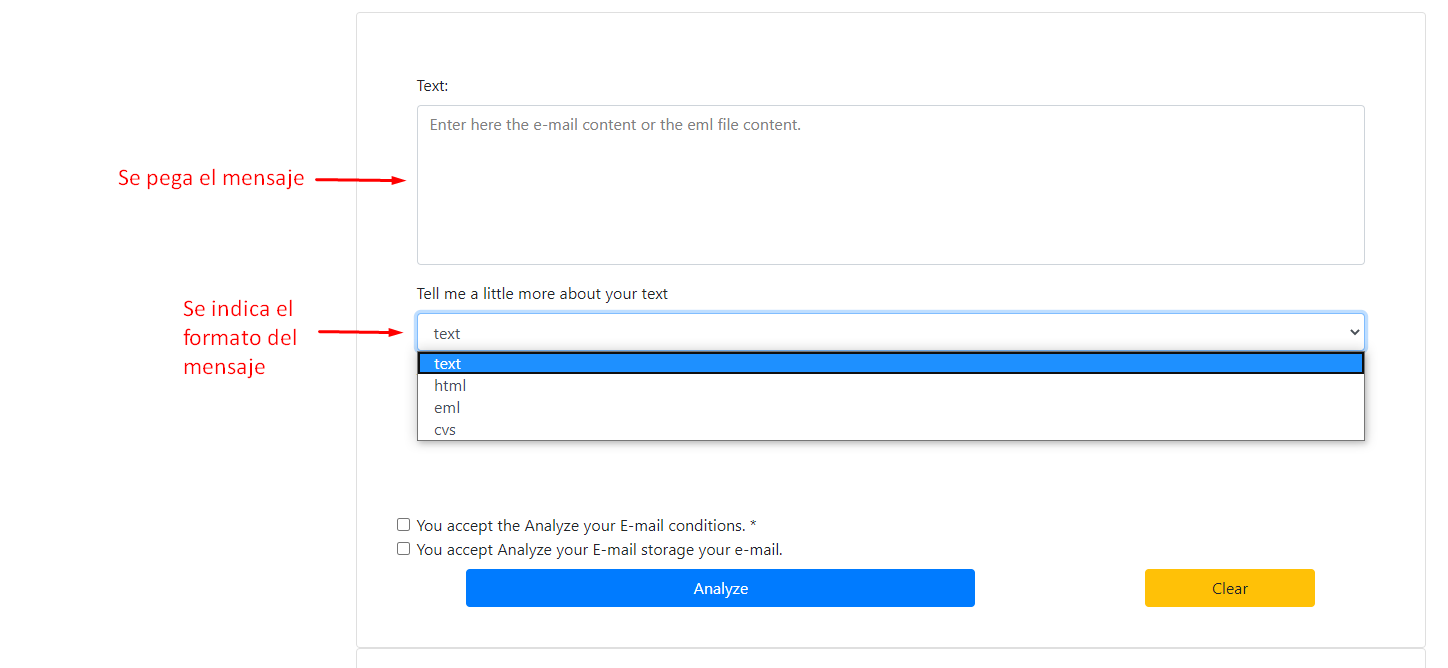
\includegraphics[width=\textwidth]{imagenes/capturasAplicacion/Analizar_mensaje.png}
\caption{Index de la aplicación}
\label{fig:index}
\end{figure}

\subsection{Mensaje}
Cuando un mensaje es analizado, el usuario verá algo parecido a las figuras \ref{fig:mensaje_datos} y \ref{fig:mensaje_patrones}. En la primera se puede ver la información básica del mensaje, como el formato, cuándo se añadió o cuándo se analizó. 

En la segunda figura \ref{fig:mensaje_patrones} se pueden ver qué patrones se han encontrado en dicho mensaje. Además, en caso de que el usuario quiera obtener más información sobre algún patrón en contro, simplemente podría clicar encima para ser redirigido a la página del patrón. 

\begin{figure}[htb]
    \centering
    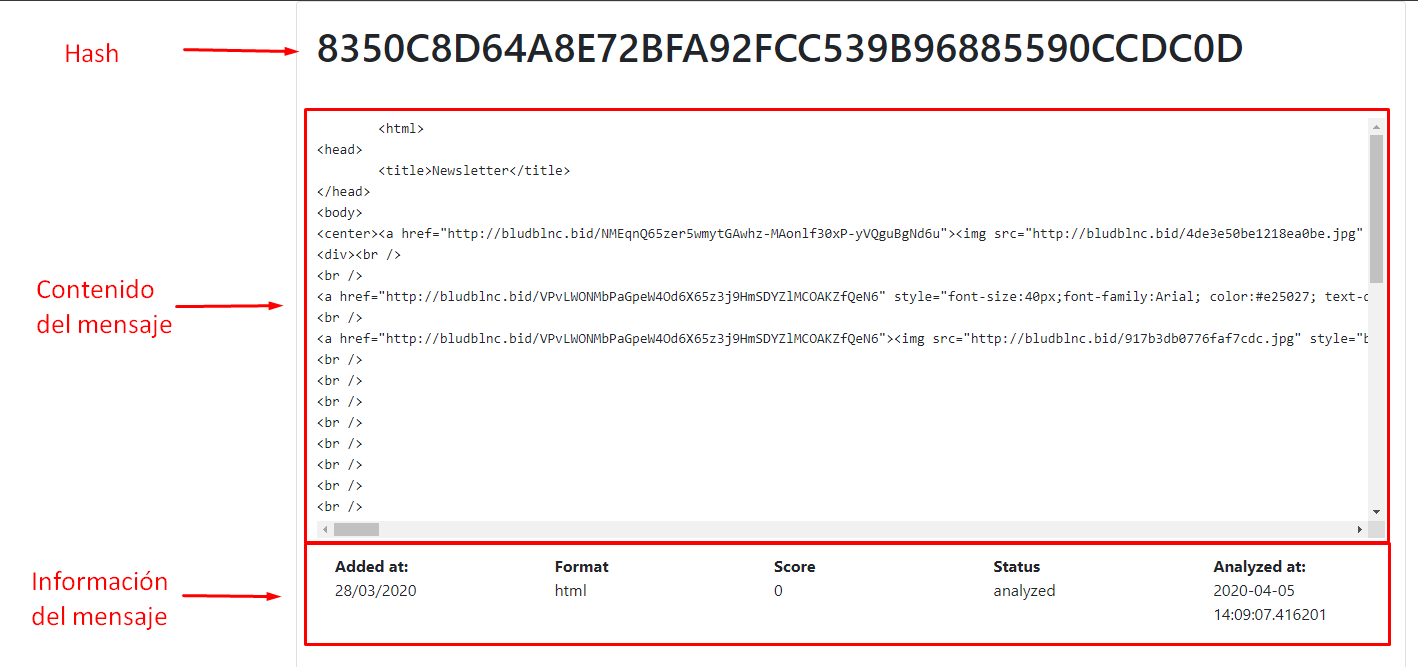
\includegraphics[width=0.8\textwidth]{imagenes/capturasAplicacion/Mensaje_info.png}
\caption{Vista de un mensaje: Información básica}
\label{fig:mensaje_datos}
\end{figure}

\begin{figure}[htb]
    \centering
    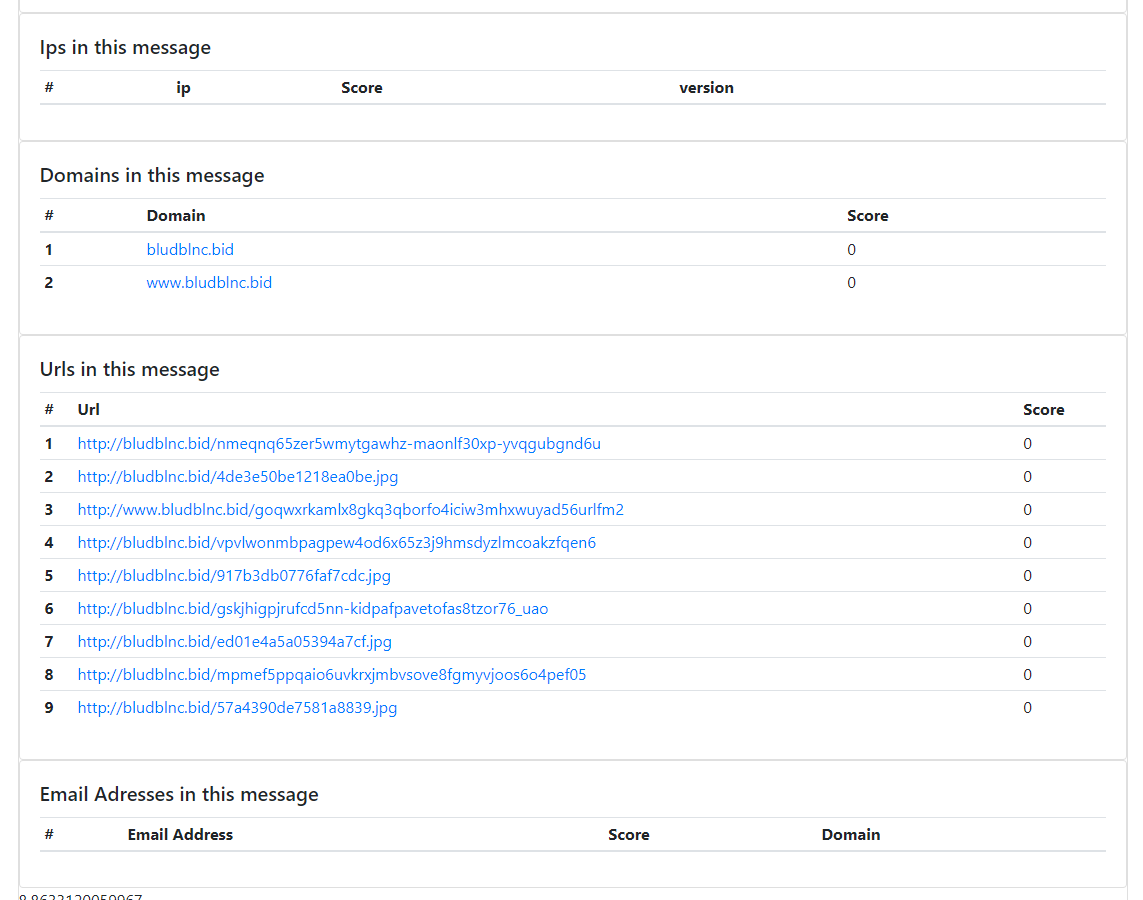
\includegraphics[width=0.8\textwidth]{imagenes/capturasAplicacion/Mensaje_patrones.png}
\caption{Vista de un mensaje: Patrones}
\label{fig:mensaje_patrones}
\end{figure}

\clearpage
\subsection{Dominio}
En el caso de los dominios, la información varía un poco dependiendo de si es un dominio (figura \ref{fig:dominio}) o un sundominio (figura \ref{fig:Subdominio}).

En caso de ser un subdominio, en la información básica aparecerá el dominio al que pertenece pudiendo navegar hacia él si se clica. 

Por otro lado, en caso de ser un dominio, aparecerán sus subdominios.

El resto de información como mensajes, enlaces, o direcciones de correo donde aparece este patrón, es idéntica y se puede navegar hacia ellos si se clica encima. 

\begin{figure}[htb]
    \centering
    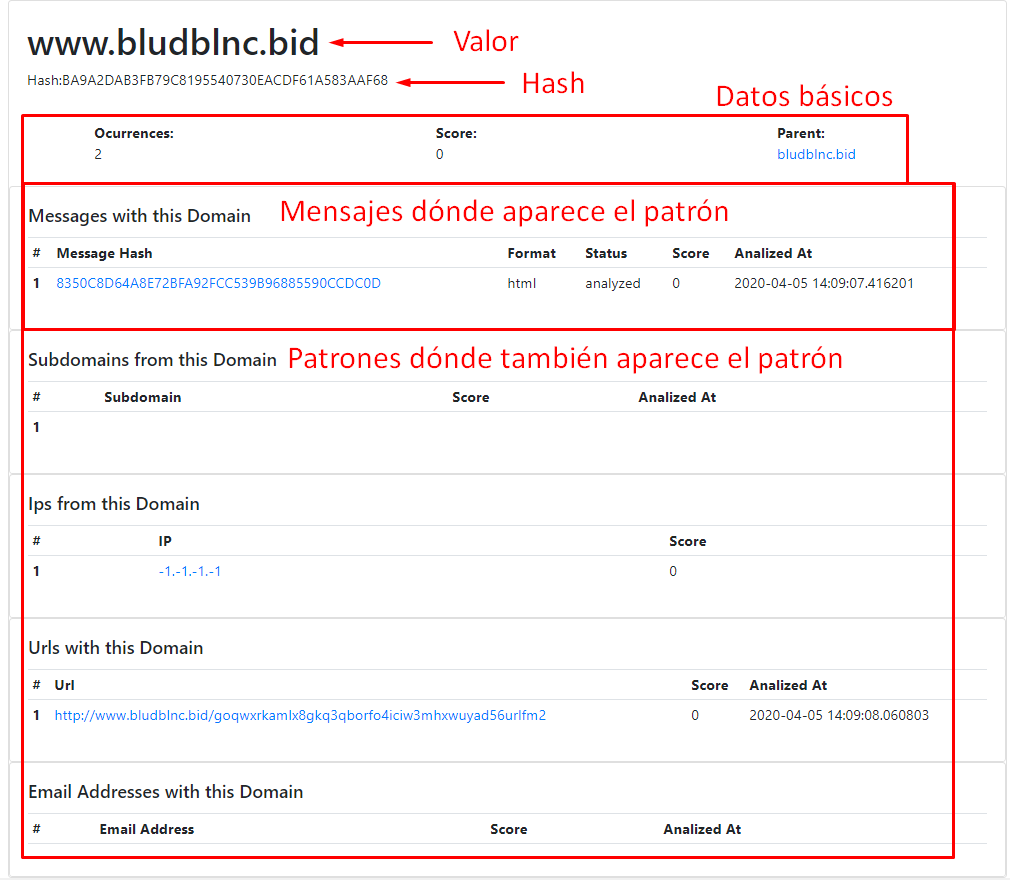
\includegraphics[width=0.9\textwidth]{imagenes/capturasAplicacion/Subdominio.png}
\caption{Vista de un subdominio.}
\label{fig:Subdominio}
\end{figure}


\begin{figure}[htb]
    \centering
    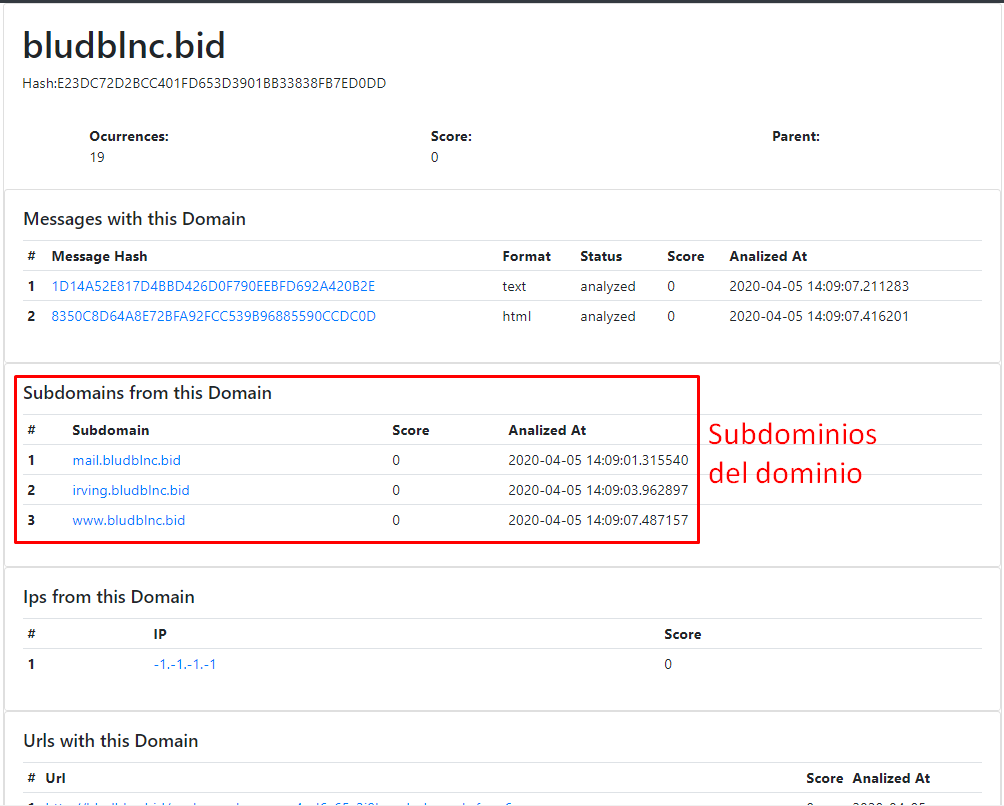
\includegraphics[width=0.9\textwidth]{imagenes/capturasAplicacion/Dominio.png}
\caption{Vista de un dominio.}
\label{fig:dominio}
\end{figure}

\clearpage
\subsection{Enlaces} \label{vista_enlaces}
En el caso de los enlaces, se ha integrado la plataforma con Virus Total, de modo que se puede analizar el enlace directamente desde la aplicación clicándo únicamente en el botón de \textit{Analyze} (Ver figuras \ref{fig:enlace} y \ref{fig:enlace_vt}).

\begin{figure}[htb]
    \centering
    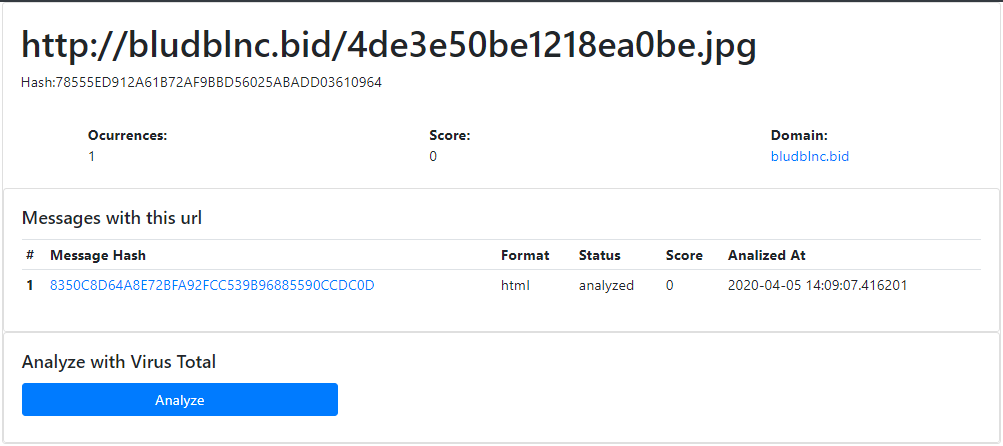
\includegraphics[width=0.8\textwidth]{imagenes/capturasAplicacion/Enlaces.png}
\caption{Vista de un enlace.}
\label{fig:enlace}
\end{figure}


\begin{figure}[htb]
    \centering
    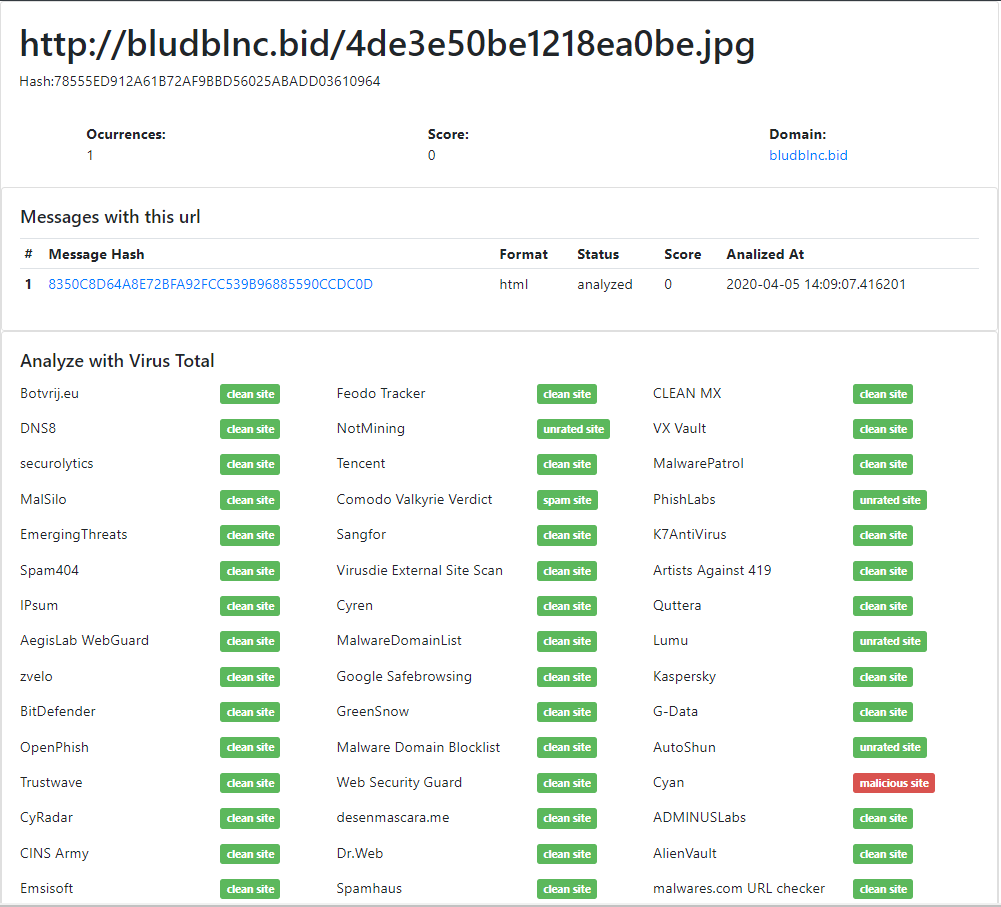
\includegraphics[width=0.8\textwidth]{imagenes/capturasAplicacion/Enlaces_virusTotal.png}
\caption{Vista de un enlace tras analizarlo con VirusTotal.}
\label{fig:enlace_vt}
\end{figure}

\clearpage
\subsection{Direcciones IP} \label{vista_ip}
Finalmente con las direcciones IP también se ha integrado el servicio de VirusTotal pudiendo analizar la dirección IP con este servicio (ver figuras \ref{fig:ip} y \ref{fig:ip_vt}).

\begin{figure}[htb]
    \centering
    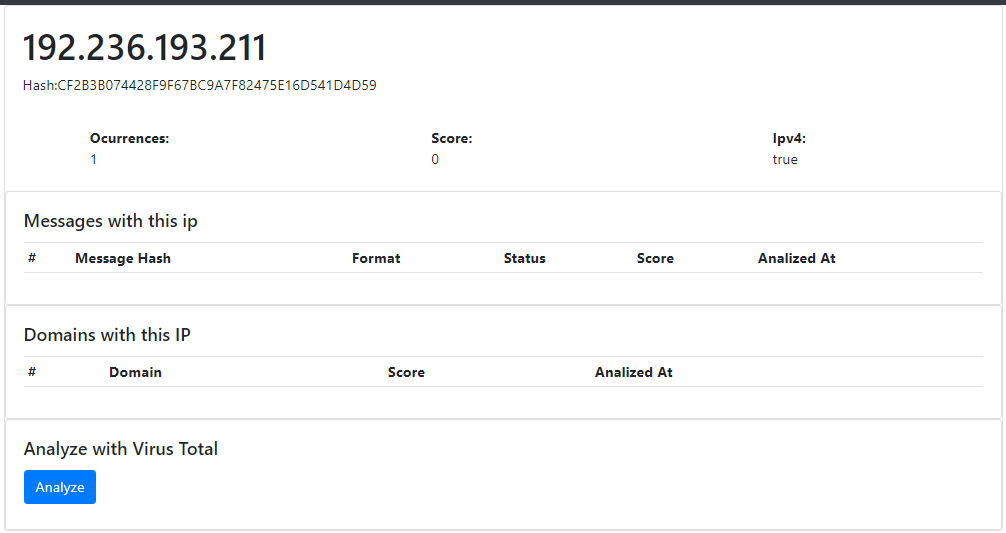
\includegraphics[width=0.8\textwidth]{imagenes/capturasAplicacion/IP.png}
\caption{Vista de una dirección IP.}
\label{fig:ip}
\end{figure}


\begin{figure}[htb]
    \centering
    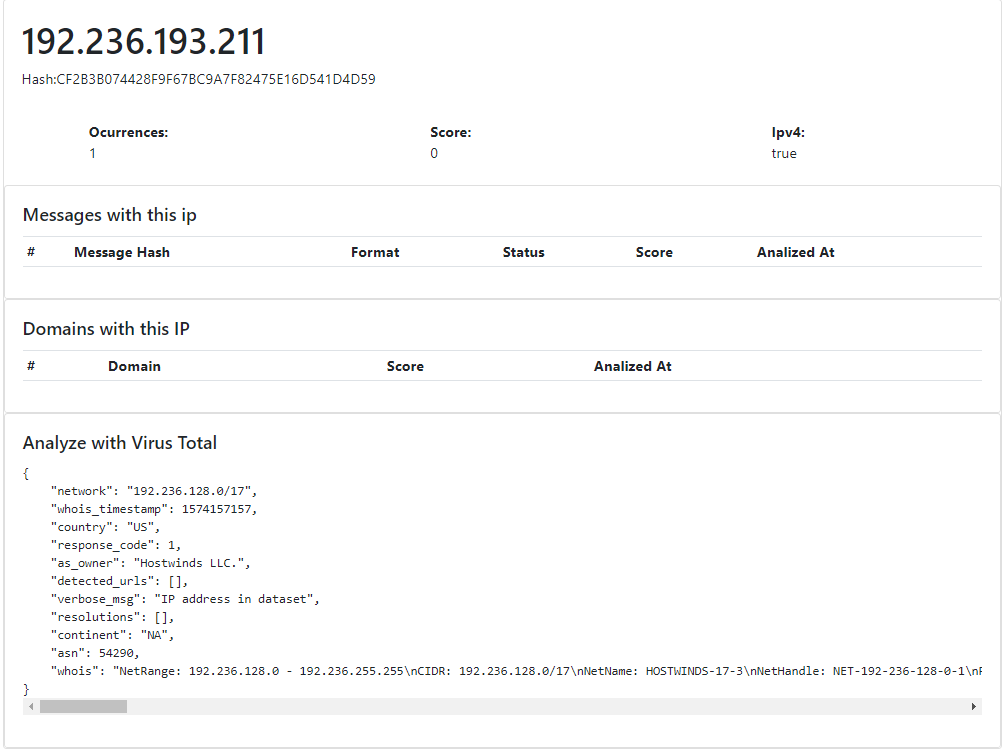
\includegraphics[width=0.8\textwidth]{imagenes/capturasAplicacion/IP_vt.png}
\caption{Vista de una dirección IP tras analizarla con VirusTotal.}
\label{fig:ip_vt}
\end{figure}
